   \pstart
Si dum pila $\displaystyle A$ provolvitur motu per detrimentum tantum alterato
interea planum eam ferens $\displaystyle BC$ progrediatur aequabili motu,
linea $\displaystyle A(A)((A))$ erit rursus logarithmica quia summae
\edtext{scilicet progressionis Geometricae terminorum}{\lemma{scilicet}\Bfootnote{\textit{(1)}\ differentiarum \textit{(2)}\ progressionis Geometricae terminorum, \textit{L}\hspace{-3mm}}},
erunt [ipsae]\edtext{}{\lemma{}\Bfootnote{ipsi \textit{\ L \"{a}ndert Hrsg.}}}
Geometricae progressionis, et haec est descriptio lineae logarithmicae physicae.
\\
\hspace*{7,5mm}
%\pend
%\pstart
Melior autem executio haec \edtext{ut in}{\lemma{ut}\Bfootnote{\textit{(1)}\ super \textit{(2)}\ in \textit{L}}}
sulcis $\displaystyle DE$, \edtext{$\displaystyle FG$ currulus}{\lemma{$\displaystyle FG$}\Bfootnote{\textit{(1)}\ cylinder \textit{(2)}\ currulus \textit{L}}}
\edtext{$\displaystyle H$ duabus rotis, compositus moveatur}{\lemma{$\displaystyle H$}\Bfootnote{\textit{(1)}\ volvatur \textit{(2)}\ duabus [...] moveatur, \textit{L}}},
et in Tabula $\displaystyle I$ recta ad sulcos perpendiculari progrediente, stylo, $\displaystyle L$ describat
\edtext{curvam $\displaystyle LP$.}{\lemma{11-S.270.1 \hspace{1.8mm}curvam $\displaystyle LP$.}\killnumber\Bfootnote{\textit{(1)}\ Sed NB non \textit{(2)}\ Linea \textit{L}}}
\pend
\vspace{1.5em}
   \pstart \noindent \centering 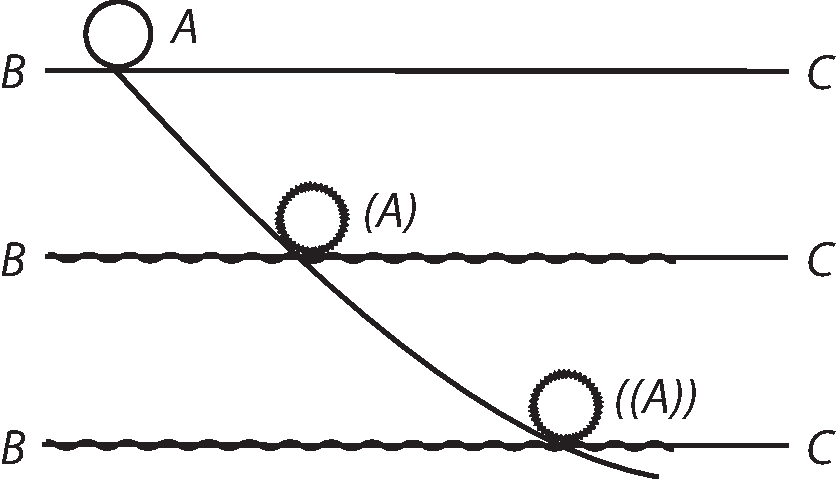
\includegraphics[trim = 0mm -3mm 0mm 0mm, clip, width=0.46\textwidth]{images/lh03705_011r-d1.pdf}\\
    \centering\setline{1}
    [\textit{Fig. 3}] % \caption{Bildbeschreibung}
    \pend
    \newpage
    \pstart
    \noindent
    \centering
      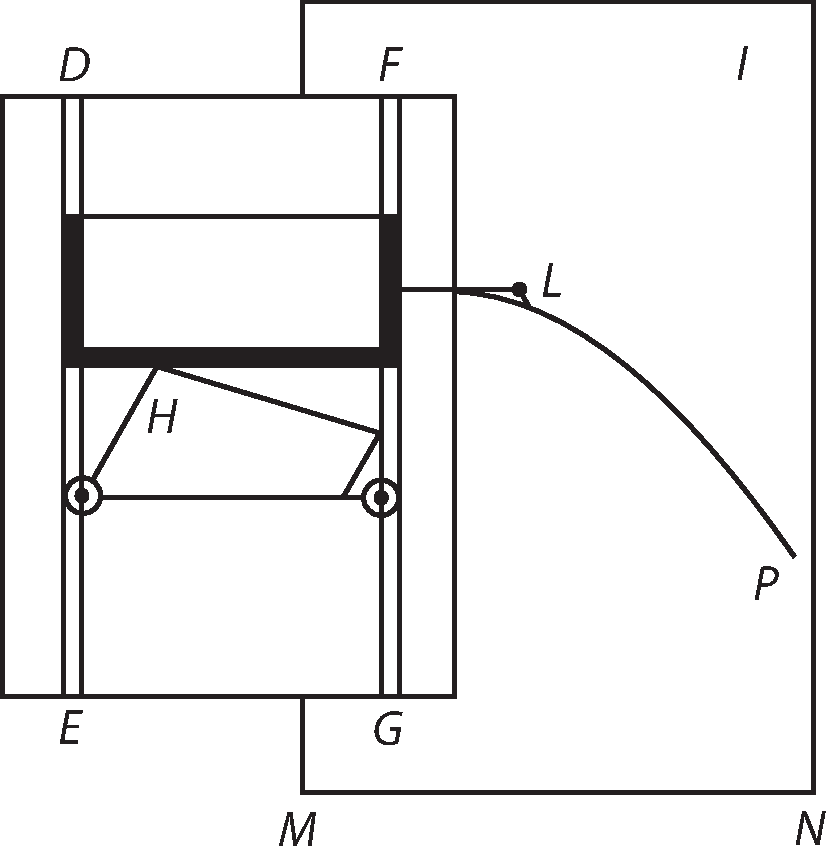
\includegraphics[trim = 0mm 0mm 0mm 0mm, clip, width=0.45\textwidth]{images/lh03705_011r-d2.pdf}\\
    \centering
    [\textit{Fig. 4}] % \caption{Bildbeschreibung}
    \pend
    \vspace{1em}
\pstart
Linea \setline{1}quae describitur motu composito ex aequabili, et continue
retardato per\textso{ Detrimentum,} est\textso{ Logarithmica.}
\pend
\count\Bfootins=1200
\count\Afootins=1200
\pstart Quae causa facit ut \edtext{corpora a motu ad quietem redeant, ea facit etiam}{\lemma{corpora}\Bfootnote{\textit{(1)}\ mota quiescant, ea facit etiam \textit{(2)}\ a motu [...] etiam \textit{L}}}
ut difficulter moveantur. Unde fit [ut]\edtext{}{\lemma{}\Bfootnote{ut\ \textit{erg. Hrsg.}}}
vi quadam opus sit, ad corpora etiam sine ulla gravitate, in plano horizontali
movenda, et eo majore, quo majus est
\edtext{corpus; objicies}{\lemma{corpus;}\Bfootnote{\textit{(1)}\ vel potius quo \textit{(2)}\ objicies \textit{L}}}
non magnitudinem corporis, sed soliditatem in quaestione esse, ex. g. libramentum
ex plumbo difficilius moveri, quam ex
\edtext{ligno; ideoque}{\lemma{ligno;}\Bfootnote{\textit{(1)}\ sed sciendum est \textit{(2)}\ ideoque \textit{L}}}
res non attritu, quia [attritus]\edtext{}{\lemma{}\Bfootnote{attritu \textit{\ L \"{a}ndert Hrsg.}}}
non est nisi superficierum. Respondeo corpora solida plus habere
etiam superficiei propriae; constant enim ex
\edtext{plurimis corpusculis}{\lemma{plurimis}\Bfootnote{\textit{(1)}\ corporibus \textit{(2)}\ corpusculis \textit{L}}}
connexis, quorum superficies medium moratur; cum porosa sint instar sylvae rarae.
Nemo negabit in \edtext{sylva densa non tantum}{\lemma{sylva}\Bfootnote{\textit{(1)}\ rara non tantum \textit{(2)}\ densa non tantum \textit{L}}}
plus ligni, sed etiam plus corticis esse quam in rara.
Ex eodem principio le trait de la balance, de qua
\edtext{Aristoteles\protect\index{Namensregister}{\textso{Aristoteles}, 384-322 v. Chr.}}{\lemma{Aristoteles}\Cfootnote{\cite{01002}\textit{Mech.} 10, 852a23-28.}}
et \edtext{Perraltus\protect\index{Namensregister}{\textso{Perrault} (Perraltus), Claude 1613-1688}}{\lemma{Perraltus}\Cfootnote{\cite{01016}C. \textsc{Perrault}, \textit{De la pesanteur des corps}, II, ch. 3, in \textit{Essais de physique}, Bd. I, Paris 1680, S. 93-97. Siehe hierzu N. 57 sowie \cite{01017}\textit{LSB} II 1, N. 128, S.~414.}},
et effectus libramenti\protect\index{Sachverzeichnis}{libramentum} (:~du balancier~:)
in horologio\protect\index{Sachverzeichnis}{horologium}, sane notabilis; idem in libramento d'un Tournebroche in gyrum acto.
\pend
\pstart
Ex his aditus aperietur ad cognoscenda quae supersunt oscillationum arcana,
nempe ut data penduli\protect\index{Sachverzeichnis}{pendulum} longitudine et pondere\protect\index{Sachverzeichnis}{pondus} annexo,
definiamus quousque prima, secunda, tertia vibratione assurgere debeat.
Quod antequam fiat, nec concursuum labyrinthi quos exhibet \edtext{Regnaldus\protect\index{Namensregister}{\textso{Regnauld} (Regnaldus), Fran\c{c}ois S.J. 1689} apud Monconisium\protect\index{Namensregister}{\textso{Monconys} (Monconisius), Balthasar de 1611-1665}}{\lemma{Regnaldus apud Monconisium}\Cfootnote{\cite{00118}F. \textsc{Regnauld}, Brief an B. de Monconys vom 21. Dezember 1655; in B. \textsc{de Monconys}, \textit{Journal des voyages}, Teil III, \textit{Lettres escrittes \`{a} Monsieur de Monconys}, Lyon 1666, S. 52-56.}} poterunt absolvi.
Item ad oscillantia Elateria\protect\index{Sachverzeichnis}{elater} poterit transferri.
Forte etiam commodior hinc reperietur mensurae universalis determinatio sine
observatione ad coelum, scilicet ut dicamus:
\edtext{pendulum, ejus}{\lemma{pendulum,}\Bfootnote{\textit{(1)}\ quod \textit{(2)}\ ejus \textit{L}}}
longitudinis (si nulla ponderis ratio, aut exigua) ut prima vibratione ad talem altitudinis
suae partem exurgat, est unius pedis, etc.
\pend
\pstart
Sed ut in accelerationem hanc gravium\protect\index{Sachverzeichnis}{acceleratio gravium} inquiramus,
vires\protect\index{Sachverzeichnis}{vis} quovis loci puncto quaesitae sunt:\edtext{}{\lemma{}\Afootnote{\textit{Am Rand:}
$\displaystyle \protect\begin{array}{llll} ab&&&\\
a^2b & ac &\\
a^3b & a^2c & ad\\
a^4b & a^3c & a^2d & ae\protect\end{array}$\\ \\ 
\hspace*{7,5mm}\textit{Dar\"{u}ber, gestrichen:}
\footnotesize
$\displaystyle \protect\begin{array}{lll} a&&\\
a^2 & b &\\
a^3 & b^2 & c\\
a^4 & b^3 & c^2 \protect\end{array}$\vspace{-6mm}}}
$\displaystyle \rule[-4mm]{0mm}{10mm} \frac{aC}{\sqrt{\vphantom{ax}}ax}$ ponendo $\displaystyle x \ \sqcap$
1 vel 2 vel 3 vel 4 etc. sive
$\displaystyle x \, \sqcap \ b + {\scriptstyle{1}} \beta$ vel $\displaystyle b + {\scriptstyle{2}} \beta$ vel $\displaystyle b + {\scriptstyle{3}} \beta$ etc. Prima ergo, si crescat celeritas, est: $\displaystyle \frac{aC}{\sqrt{ab + a \beta}} + C$. Resistentia erit $\displaystyle \frac{\beta a C}{r \sqrt{ab + a \beta}} + \frac{\beta}{r} C$
\pend
%\newpage
\count\Bfootins=1500
\count\Afootins=1500
\pstart
\noindent
et residua vis erit $\displaystyle \rule[-4mm]{0mm}{10mm} \frac{a}{\sqrt{ab + a \beta}} + 1, \, \smallfrown C,\!, \, \smallfrown 1 - \frac{\beta}{r}$.
Cui addatur $\displaystyle \frac{a}{\sqrt{ab + 2a \beta}} C$,
fiet $\displaystyle \frac{a}{\sqrt{ab + a \beta}} + 1, \, \smallfrown \, 1 - \rule[-4mm]{0mm}{10mm} \frac{\beta}{r},\!, \, + \ \frac{a}{\sqrt{ab + 2a \beta}},\!,\!, \, [\smallfrown] \ 1 - \frac{\beta}{r},\!,\!,\!, \, \smallfrown \, C$\edtext{}{\lemma{}\Bfootnote{$\displaystyle \smallfrown$ \textit{\ erg. Hrsg.}}} residua vis.
Itaque hinc jam patet series[:]
$\begin{array}{llllll}
I) 
& {\displaystyle 1 + \frac{a}{\sqrt{ab + a \beta}}} 
& {\displaystyle \smallfrown 1 - \frac{\beta}{r}}
\\
II) 
& \multicolumn{1}{c}{\displaystyle \dotfill}
& {\displaystyle \smallfrown {\atop \lefthalfcup} 1 - \frac{\beta}{r} {\atop \righthalfcup}}
& \overset{\displaystyle 2}{\displaystyle \cdot}
& {\displaystyle \pm  \frac{a}{\sqrt{ab + 2a \beta}} \smallfrown 1 - \frac{\beta}{r}}
\\
III) 
& \multicolumn{2}{c}{\displaystyle \dotfill} 
& \overset{\displaystyle 3}{\displaystyle \cdot}
& \multicolumn{1}{c}{\displaystyle \dotfill} 
& {\displaystyle \overset{\displaystyle 2}{\displaystyle \cdot} \ \ \pm \frac{a}{\sqrt{ab + 3a \beta}} \smallfrown 1 - \frac{\beta}{r}.}
\\
\end{array}$
\\
\pend
%\newpage
\pstart
   \noindent Breviter \setline{4}sic enuntiabitur: termino dato, addatur terminus respondens seriei $\displaystyle \rule[-4mm]{0mm}{10mm} \frac{a \beta}{\sqrt{ab + ax}}$
productum multiplicetur per $\displaystyle 1 - \frac{\beta}{r}$.
%Iam \edtext{auferatur}{\lemma{}\Bfootnote{auferatur \textit{erg.} \textit{L}}}
%$\displaystyle AB$ vocetur ut \edtext{superiore scheda}{\lemma{superiore scheda}\Cfootnote{Siehe \cite{?????}N. ??R/2\textsubscript{2}, S. ?? [[35.7,12v]].}},
%terminus sequens $\displaystyle CD$, terminus
%\edtext{datus. $\displaystyle CF$ producta}{\lemma{datus.}\Bfootnote{\textit{(1)}\ Etsi differentia terminorum \textit{(2)}\ $\displaystyle CF$ producta \textit{L}\hspace*{14mm}}},
%erit $\displaystyle AB \, \sqcap \, CD \, (\leibdashv) \, \rule[-4mm]{0mm}{10mm} \frac{CD}{CF} \beta$
%generaliter
%    at in nostro casu
%$\displaystyle AB \, \sqcap \, CD \, \leibvdash \, CD \rule[-4mm]{0mm}{10mm} \frac{\beta}{r} \leibdashv \frac{a \beta}{\sqrt{ab + ax}} \leibvdash \frac{a \beta^2}{r \sqrt{ab + ax}}$
%deleatur terminus in quo $\displaystyle \beta^2$
%fiet
%$\displaystyle (\leibdashv) \rule[-4mm]{0mm}{10mm} \frac{CD}{CF} \, \sqcap \,
% \leibvdash \, \frac{CD}{r} \, \leibdashv \frac{a}{\sqrt{ab + ax}}$
%et fiet
%\rule[-4mm]{0mm}{10mm} \edtext{$\displaystyle CF \sqcap \frac{CDr \sqrt{ab + ax}}{\leibvdash \, CD \sqrt{ab + ax} \, \leibdashv \, ar}$. Et facile}{\lemma{$\displaystyle CF \sqcap \frac{CDr \sqrt{ab + ax}}{\leibvdash \, CD \sqrt{ab + ax} \, \leibdashv \, ar}$.}\Bfootnote{\textit{(1)}\ Problemata \textit{(2)}\ Et facile \textit{L}}}\rule[-4mm]{0mm}{10mm} patet eodem modo institui calculum si pro
%$\displaystyle \rule[-4mm]{0mm}{10mm}  \frac{aC}{\sqrt{ab + ax}}$ alia substituta
%\edtext{fuisset figurae analyticae ordinata}{\lemma{fuisset}\Bfootnote{\textit{(1)}\ series \textit{(2)}\ figurae analyticae ordinata \textit{L}}},
%itaque semper res redit ad hoc problema:
Iam \edtext{auferatur}{\lemma{}\Bfootnote{auferatur \textit{erg. L}}}
$\displaystyle AB$ vocetur ut \edlabel{037,05_011r_scheda-1}\edtext{superiore scheda,}{\lemma{superiore scheda}\Cfootnote{Vermutlich N.~31\textsubscript{2}.}}\edlabel{037,05_011r_scheda-2} terminus sequens $\displaystyle CD,$ terminus
\edtext{datus. $\displaystyle CF$ producta,}{\lemma{datus.}\Bfootnote{\textit{(1)}\ Etsi differentia terminorum \textit{(2)}\ $\displaystyle CF$ producta, \textit{L}\hspace*{14mm}}}
erit $\displaystyle AB \, \sqcap \, CD \, (\pleibdashv\displaystyle\!) \, \rule[-4mm]{0mm}{10mm} \frac{CD}{CF} \beta$
generaliter[,] at in nostro casu
$\displaystyle AB \, \sqcap \, CD \ \pleibvdash\displaystyle \, CD \rule[-4mm]{0mm}{10mm} \frac{\beta}{r} \, \pleibdashv\displaystyle \frac{a \beta}{\sqrt{ab + ax}}\, \pleibvdash\displaystyle \frac{a \beta^2}{r \sqrt{ab + ax}}$
deleatur terminus in quo $\displaystyle \beta^2$
fiet
$\displaystyle (\pleibdashv\displaystyle\!)\, \rule[-4mm]{0mm}{10mm} \frac{CD}{CF} \, \sqcap \
 \pleibvdash\displaystyle \frac{CD}{r} \, \pleibdashv\displaystyle \frac{a}{\sqrt{ab + ax}}$
et fiet
$\displaystyle CF \sqcap
\rule[-4mm]{0mm}{10mm}\edtext{\frac{CDr \sqrt{ab + ax}}{\efrac{}{\leibvdash\displaystyle} CD \sqrt{ab + ax} \, \efrac{}{\leibdashv\displaystyle}\, ar}$.
Et facile}{\lemma{$\displaystyle\frac{CDr \sqrt{ab + ax}}{\efrac{}{\leibvdash\displaystyle} CD \sqrt{ab + ax} \, \efrac{}{\leibdashv\displaystyle}\, ar}$.}\Bfootnote{\textit{(1)}\ Problemata \textit{(2)}\ Et facile \textit{L}}}\rule[-4mm]{0mm}{10mm} patet eodem modo institui calculum si pro
$\displaystyle \rule[-4mm]{0mm}{10mm}  \frac{aC}{\sqrt{ab + ax}}$
\rule[-4mm]{0mm}{10mm}alia substituta
\edtext{fuisset figurae analyticae ordinata}{\lemma{fuisset}\Bfootnote{\textit{(1)}\ series \textit{(2)}\ figurae analyticae ordinata, \textit{L}}},
\pend
\vspace{0.9em}
\pstart
\noindent
\centering
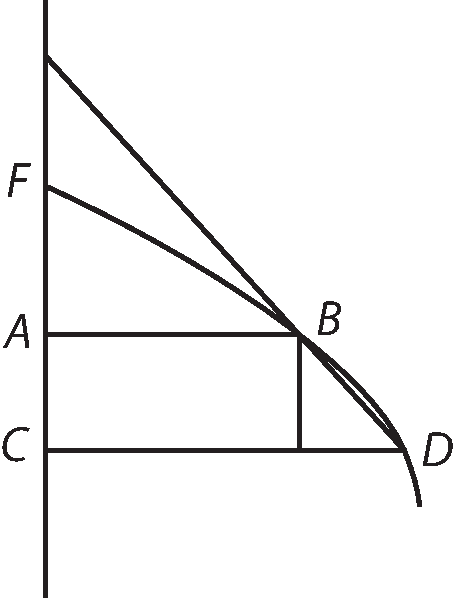
\includegraphics[trim = 0mm -1mm 0mm 0mm, clip,width=0.24\textwidth]{images/lh03705_011r-d3.pdf}\\
\centering
\setline{11} [\textit{Fig. 5}] % \caption{Bildbeschreibung}
\pend
\newpage
\pstart
\noindent
itaque semper res redit ad hoc problema:
Data producta, invenire figuram, quotiescunque de motus detrimento quaeritur,
\edtext{modo incrementa}{\lemma{modo}\Bfootnote{\textit{(1)}\ series \textit{(2)}\ incrementa \textit{L}}}
celeritatum vel decrementa, in quovis spatii puncto
\edtext{analytice habeantur}{\lemma{}\Bfootnote{analytice  \textbar\ vel saltem ex datis quoque praestita \textit{gestr.}\ \textbar\ habeantur. \textit{L}}}.
   Imo male. $\displaystyle CD$ non est constans sed variabilis
itaque intererit[;] ipsam $\displaystyle \rule[-4mm]{0mm}{10mm}  \frac{aC}{\sqrt{ab + ax}}$
etiam ita resolvi, ut ex unica pendeat sequentes scilicet ex antecedente.  [11~v\textsuperscript{o}]
\pend
\count\Bfootins=1500
\count\Afootins=1500
\count\Cfootins=1500

